\documentclass[conference]{IEEEtran}
\usepackage{graphicx}
\usepackage{booktabs}
\usepackage{amsmath}
\usepackage{url}
\usepackage[hidelinks]{hyperref}
\usepackage{cite}

\begin{document}

\title{Where Do Layout Detectors Fail on Indian Documents?\\ A Study of Script, Domain and Scan Quality on IndicDLP}

\author{
\IEEEauthorblockN{Prashant Jha, Aditya Soni, Riddhi Patil and Mariam Badure}
\IEEEauthorblockA{Department of Artificial Intelligence and Machine Learning\\
St. Francis Institute of Technology (Autonomous), Mumbai, India\\
Project guide: Dr.~Joanne Gomes}
}

\maketitle

\begin{abstract}
Layout detection, finding the paragraphs, headings, tables and other regions on a page, is the first step in reading scanned documents. Strong detectors for Indian-language documents now exist, so instead of proposing another one we study where they fail. On 682 held-out pages of the IndicDLP dataset (12 languages, 12 document types, 42 region labels) we compare the released DocLayout-YOLO model with a YOLOv8s and a Faster R-CNN that we fine-tuned on a laptop budget, and we define three simple measures: a Consistency Index and a Robustness Index. The released model reaches 0.759 mAP@50, against 0.259 and 0.148 for our models. Its accuracy is even across languages (CI 0.86) but not across document types (CI 0.55; forms are hardest). Under five kinds of scan damage it keeps 97\% of its accuracy on average; blur hurts most. For text reading, choosing the OCR language by probing detected regions is right on 106 of 120 pages, against 70 for Tesseract's built-in detector. We release the data subset as CSV files, the code, and IndicDoc AI, a web app and API that detects regions and reads text in 12 Indian languages.
\end{abstract}

\begin{IEEEkeywords}
document layout analysis, Indian languages, object detection, robustness, cross-script generalisation, OCR
\end{IEEEkeywords}

\section{Introduction}
India has 22 scheduled languages written in about a dozen scripts. Government offices, courts, schools and
newspapers hold millions of scanned pages in these languages. To search such a page, or to read it aloud for a
visually impaired person, a computer must first find the parts of the page --- paragraphs, headings, tables,
figures, page numbers --- and only then read the text inside each part. This first step is called
\emph{document layout analysis}. If it goes wrong, every later step (OCR, table extraction, question answering)
goes wrong too.

Most layout datasets and tools are built for English. The recent IndicDLP dataset~\cite{indicdlp} changed this: it
has about 120{,}000 human-labelled pages in 12 Indian languages and 12 document types, and its authors showed that
modern detectors such as YOLOv10 and DocLayout-YOLO~\cite{doclayout} reach about 55 mAP@50:95 on it. They also
reported that accuracy drops by 20--25 points on scripts the model has not seen.

Strong detectors therefore already exist. We do \textbf{not} propose a new detector. Instead, we ask a simpler
and, we believe, more useful question for people who want to \emph{use} these detectors on real Indian documents:
\textbf{where and why do they fail?} We study this with five research questions:
\begin{itemize}
\item \textbf{RQ1} How far behind is a detector trained on a small compute budget, compared with one trained on the full dataset?
\item \textbf{RQ2} Is accuracy even across the 12 languages and the 12 document domains?
\item \textbf{RQ3} Which region types are hardest, and is this because they are rare in the training data?
\item \textbf{RQ4} How much accuracy survives common scan damage: blur, noise, heavy JPEG compression, low resolution and faded print?
\item \textbf{RQ5} Can the detected regions be used to choose the right OCR language automatically?
\end{itemize}

\noindent Our contributions are:
\begin{enumerate}
\item A controlled comparison of three detectors (the released IndicDLP DocLayout-YOLO, and a YOLOv8s and a Faster
R-CNN that we fine-tuned) on the same 682 held-out test pages.
\item Two simple summary measures that can be reported next to mAP: the \emph{Consistency Index} (CI) and the
\emph{Robustness Index} (RI).
\item The first (to our knowledge) scan-damage robustness test on IndicDLP.
\item IndicDoc AI, an open tool (web app, REST API, Docker) that detects regions on Indian-language pages and reads
their text with automatic script selection, built on the best detector of the study.
\end{enumerate}

\section{Related Work}
\textbf{Indian-language layout datasets.} IndicDLP~\cite{indicdlp} provides 119{,}806 pages, 12 languages, 12
domains and 42 region labels, and benchmarks six detectors (YOLOv10x, DocLayout-YOLO, RoDLA, DINO, DiT,
Florence-2). The best models are vision-only and reach about 55 mAP@50:95; the paper does not test damaged scans.
UniTabBank~\cite{unitabbank} covers tables in 28 languages and reports that borderless tables and degraded scans
remain hard.

\textbf{Detectors.} Faster R-CNN~\cite{fasterrcnn} is a classic two-stage detector: it first proposes regions,
then classifies them. YOLO detectors~\cite{yolov8} are one-stage and much faster. DocLayout-YOLO~\cite{doclayout}
adapts YOLOv10 to documents with a global-to-local receptive-field module and synthetic pre-training data.

\textbf{Text recognition and understanding for Indian scripts.} PLATTER~\cite{platter} detects and recognises
handwritten Indic words but needs the user to name the language. HindiOCR-VLM~\cite{hindiocr} fine-tunes a
vision-language model for Hindi only. LayoutXLM~\cite{layoutxlm} joins text, layout and image but covers no Indian
language. DRISHTIKON~\cite{drishtikon} grounds answers on the page and depends on OCR blocks. Table QA for Bengali
and Hindi~\cite{tableqa} and Devanagari table extraction~\cite{devtables} both assume that tables have already
been found. All of these works need a reliable layout step first, which motivates our study.

\textbf{Robustness.} Hendrycks and Dietterich~\cite{hendrycks} showed that image classifiers lose much accuracy
under common corruptions such as blur, noise and JPEG compression. We apply the same idea to Indian document
layout detection.

\section{Data and Models}
\subsection{Dataset}
We use a language-balanced subset of IndicDLP (MIT licence), taken from the official train, validation and test
splits so that no test page was used for training by us or by the dataset authors. We stream only the needed
parts of the Parquet files from Hugging Face, convert them to COCO JSON, clip boxes to the page and drop boxes
smaller than one pixel (0.5\% of training boxes). Table~\ref{tab:data} gives the sizes. The subset is released as
CSV files (pages, boxes, class counts) with the code.

\begin{table}[t]
\centering
\caption{Our IndicDLP subset (pages).}
\label{tab:data}
\small
\begin{tabular}{lrrr}
\toprule
Language & Train & Val & Test \\
\midrule
Assamese & 129 & 30 & 60 \\
Bengali & 200 & 30 & 60 \\
English & 188 & 30 & 60 \\
Gujarati & 200 & 30 & 60 \\
Hindi & 200 & 21 & 22 \\
Kannada & 200 & 21 & 60 \\
Malayalam & 200 & 30 & 60 \\
Marathi & 200 & 30 & 60 \\
Odia & 200 & 30 & 60 \\
Punjabi & 188 & 30 & 60 \\
Tamil & 200 & 30 & 60 \\
Telugu & 188 & 30 & 60 \\
\midrule
\textbf{Total} & \textbf{2,293} & \textbf{342} & \textbf{682} \\
Boxes & 33,667 & 5,815 & 10,513 \\
\bottomrule
\end{tabular}
\end{table}

The label distribution is very uneven: \emph{paragraph} alone is 32\% of all boxes, and 10 of the
42 labels have fewer than 100 training boxes.

\subsection{Models}
\textbf{DocLayout-YOLO (released).} The checkpoint published by the IndicDLP authors (Zenodo 15881917, CC-BY 4.0),
trained on the full IndicDLP training split (about 96K pages) at 1024 pixels; 20.0M parameters. We use it
exactly as released.

\textbf{YOLOv8s (ours).} COCO-pretrained, with a new 42-class head, fine-tuned on our 2,293 training pages
at 640 pixels, batch 8, for a one-hour budget (12 epochs) on an Apple M1 Pro GPU. Mosaic, colour and scale
augmentation are used; horizontal flips are turned off because a mirrored page is not a realistic document;
11.2M parameters.

\textbf{Faster R-CNN (ours).} ResNet-50 FPN, COCO-pretrained, new 43-output predictor (42 labels and background),
SGD (learning rate 0.005, momentum 0.9, weight decay $5\times10^{-4}$, cosine schedule), batch 4, 2 epochs in 76
minutes on the same GPU; 41.5M parameters.

\section{Study Design}
\subsection{Measures}
All detectors are scored with COCO~\cite{coco} mAP@50 and mAP@50:95 (pycocotools, up to 300 boxes per page), and with
precision, recall and F1 at a fixed confidence. On top of mAP we define two simple numbers. Each is a ratio
between 0 and (about) 1, where 1 is best.

\textbf{Consistency Index.} For a set of groups $G$ (languages or domains),
\begin{equation}
\mathrm{CI} = \frac{\min_{g \in G} \mathrm{mAP}_{50}(g)}{\max_{g \in G} \mathrm{mAP}_{50}(g)}.
\end{equation}
CI $=1$ means every group is served equally well.

\textbf{Robustness Index.} For a type of damage $c$,
\begin{equation}
\mathrm{RI}_c = \frac{\mathrm{mAP}_{50}(\text{damaged by } c)}{\mathrm{mAP}_{50}(\text{clean})}.
\end{equation}
RI $=0.9$ means the detector keeps 90\% of its accuracy on that kind of page.

\subsection{Experiments}
\textbf{E1 (RQ1--RQ3).} All three detectors on the 682 clean test pages, with results broken down by
language, domain and label.

\textbf{E2 (RQ4).} The same test pages damaged in five ways that are common in real scans and phone photos
(Table~\ref{tab:corr}). Each damaged copy is made once with a fixed random seed, and the boxes stay the same.

\begin{table}[t]
\centering
\caption{Scan damage used in E2.}
\label{tab:corr}
\small
\begin{tabular}{ll}
\toprule
Damage & How it is made \\
\midrule
Blur & Gaussian blur, radius 2 px (out of focus) \\
Noise & Gaussian noise, $\sigma = 20$ grey levels (grain) \\
JPEG & JPEG quality 15 (forwarded phone image) \\
Half resolution & down to 50\%, back up (low-dpi scan) \\
Faded print & contrast $\times 0.45$, brightness $\times 1.25$ \\
\bottomrule
\end{tabular}
\end{table}

\textbf{E3 (RQ5).} On 120 test pages (10 per language) we compare two ways of choosing the OCR language:
Tesseract's built-in script detector (OSD), and our region probe, which reads one detected text region with
each of the 12 script models and counts only the characters that belong to that model's own script.


\section{Results}

\begin{table*}[t]
\centering
\caption{RQ1: the three detectors on the same 682 test pages. P/R/F1 at the confidence with the best F1 on the
validation pages. Time per page on an Apple M1 Pro GPU.}
\label{tab:overall}
\small
\setlength{\tabcolsep}{3.2pt}
\begin{tabular}{lcccccc}
\toprule
Model & mAP$_{50}$ & mAP$_{50:95}$ & P & R & F1 & s/page \\
\midrule
DocLayout-YOLO (released) & 0.759 & 0.575 & 0.848 & 0.775 & 0.810 & 0.150 \\
YOLOv8s (ours) & 0.259 & 0.165 & 0.603 & 0.508 & 0.551 & 0.024 \\
Faster R-CNN (ours) & 0.148 & 0.079 & 0.510 & 0.435 & 0.469 & 0.202 \\
\bottomrule
\end{tabular}
\end{table*}

\subsection{RQ1: small budget versus full training}
Table~\ref{tab:overall} shows a large gap. The released DocLayout-YOLO reaches 0.759 mAP@50 (the IndicDLP paper
reports about 0.735 on its full test set, so our test subset is of similar difficulty). Our YOLOv8s, trained for
one hour on 2,293 pages, reaches 0.259, and our Faster R-CNN 0.148. The one-stage YOLOv8s is better than the two-stage
Faster R-CNN with the same data and similar time, and 9$\times$ faster per page. In the
``find every part'' setting (confidence 0.15, chosen on validation pages so that precision stays at least 0.70),
the released model finds 85\% of all labelled regions at 74\% precision.

\textbf{Answer.} A detector trained on a laptop budget is about 2.9$\times$ worse in mAP@50 than one trained on
the full data (about 42$\times$ more pages). For practical use the released model should be used, which is what
our tool does.

\begin{figure*}[t]
\centering
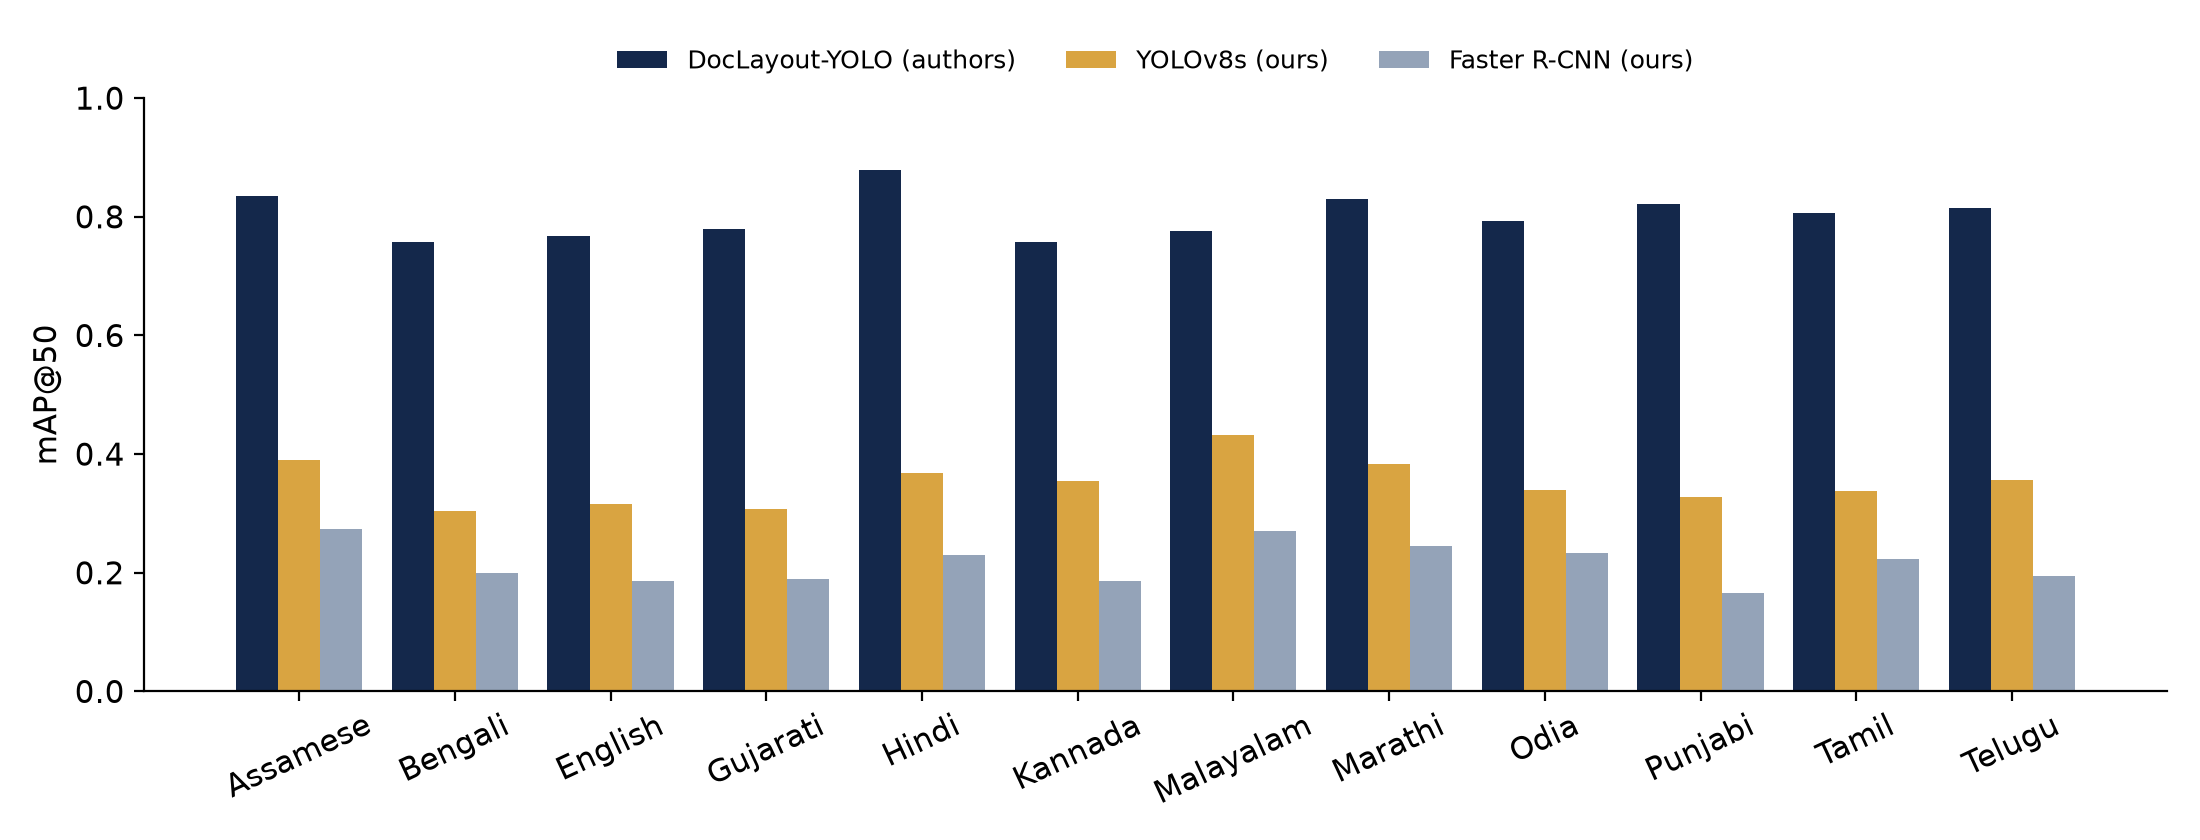
\includegraphics[width=0.92\textwidth]{figures/fig_per_language.png}
\caption{RQ2: mAP@50 per language for the three detectors.}
\label{fig:lang}
\end{figure*}

\begin{table}[t]
\centering
\caption{RQ2: mAP@50 per document domain, and the Consistency Index (CI) over languages and over domains.}
\label{tab:domain}
\small
\setlength{\tabcolsep}{4pt}
\begin{tabular}{lrcc}
\toprule
Domain & Pages & DocLayout-YOLO & YOLOv8s \\
\midrule
Research papers & 68 & 0.889 & 0.402 \\
Acts \& rules & 68 & 0.856 & 0.427 \\
Textbooks & 62 & 0.838 & 0.455 \\
Question papers & 40 & 0.837 & 0.317 \\
Syllabi & 54 & 0.833 & 0.282 \\
Manuals & 58 & 0.823 & 0.339 \\
Notices & 36 & 0.795 & 0.324 \\
Newspapers & 36 & 0.778 & 0.224 \\
Novels & 69 & 0.753 & 0.503 \\
Brochures & 66 & 0.716 & 0.260 \\
Magazines & 79 & 0.604 & 0.255 \\
Forms & 46 & 0.485 & 0.153 \\
\midrule
CI over 12 languages & & 0.86 & 0.70 \\
CI over 12 domains & & 0.55 & 0.30 \\
\bottomrule
\end{tabular}
\end{table}

\subsection{RQ2: languages and domains}
Across the 12 languages the released model ranges from 0.757 (Bengali) to 0.879 (Hindi, only 22 pages), a language Consistency Index of
0.86 (Fig.~\ref{fig:lang}). Across the 12 \emph{domains} the spread is much larger: from 0.485 on forms to 0.889 on
research papers, a domain CI of only 0.55 (Table~\ref{tab:domain}). Forms, with many small fields and boxes, and magazines, with
free designs, are the hardest; research papers and acts with regular columns are the easiest. The same pattern
holds for our two models.

\textbf{Answer.} Once a model has seen a script, the \emph{kind of document} matters more than the
\emph{language}. Reporting only one overall mAP hides that forms are served much worse than research papers.

\begin{figure*}[t]
\centering
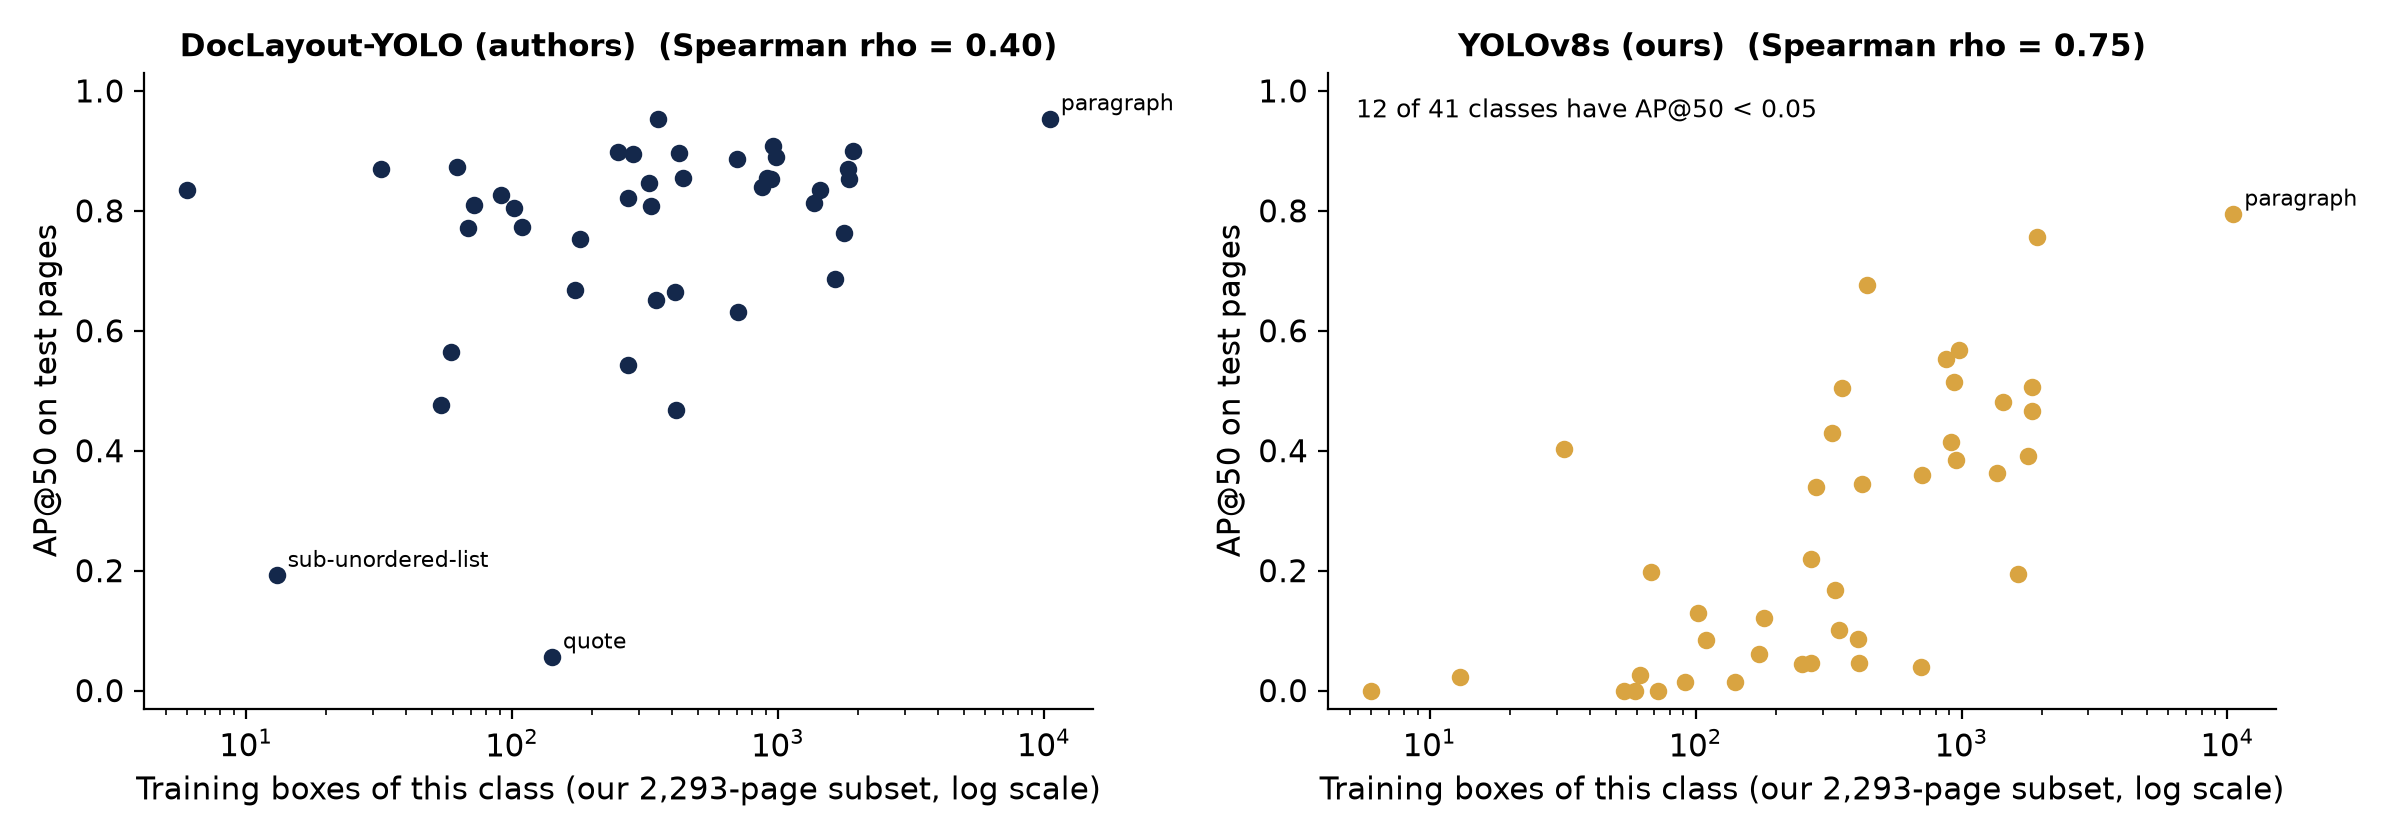
\includegraphics[width=0.92\textwidth]{figures/fig_class_frequency.png}
\caption{RQ3: AP@50 of each label against how many training boxes it has in our subset (log scale).}
\label{fig:class}
\end{figure*}

\subsection{RQ3: hard labels}
For the released model the easiest labels are \emph{paragraph} (0.95), \emph{advertisement} (0.95), \emph{ordered-list} (0.91), \emph{figure} (0.90); the hardest are \emph{quote} (0.06), \emph{sub-unordered-list} (0.19), \emph{sub-section-title} (0.47), \emph{subsub-headline} (0.48) (Fig.~\ref{fig:class}). Hard labels are
mostly nested or look-alike structures (a sub-list inside a list, a sub-section title next to a section title)
or rare ones such as quotes. For our YOLOv8s, the rank correlation between how often a label appears in training
and its AP is $\rho = 0.75$; for the released model, trained on about 42$\times$ more pages, it falls to $\rho = 0.40$.

\textbf{Answer.} With little data, rarity is the main reason a label fails. With full data, rarity matters much
less and the remaining errors come from labels that look alike and differ only by their nesting.

\begin{figure*}[t]
\centering
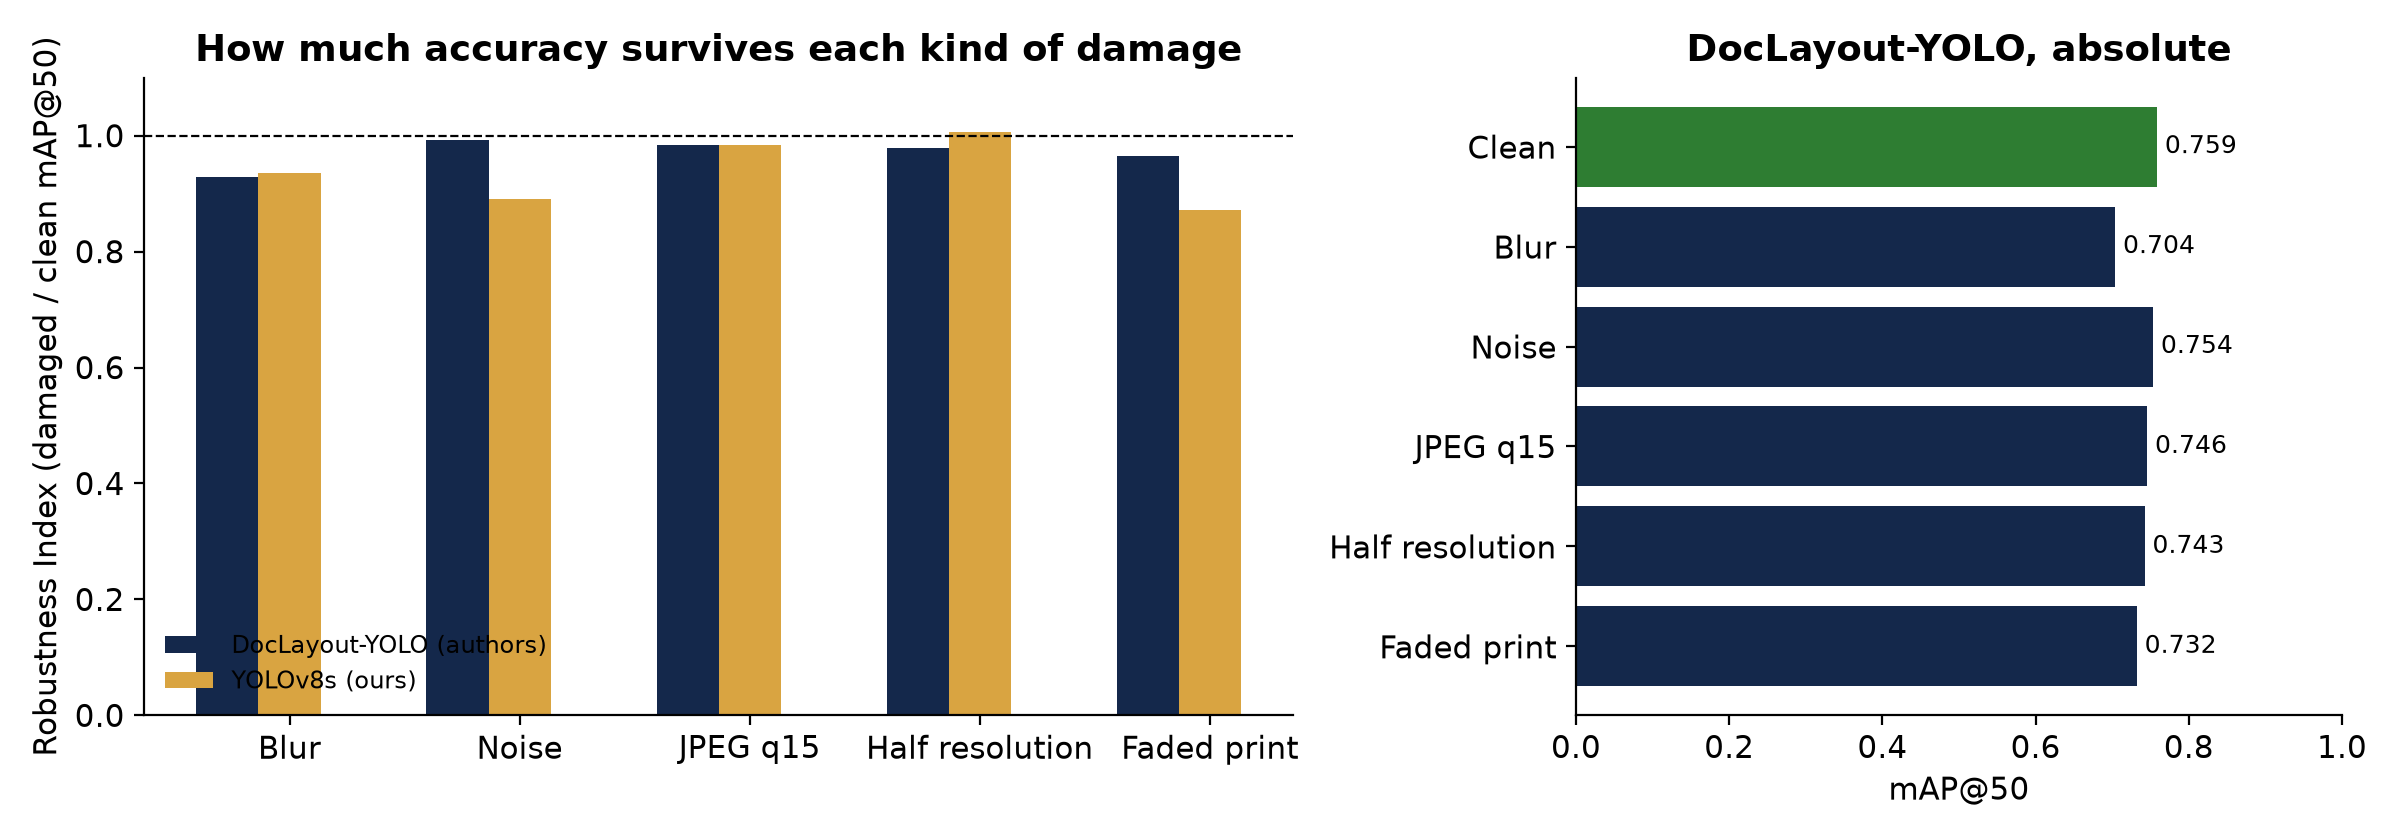
\includegraphics[width=0.92\textwidth]{figures/fig_robustness.png}
\caption{RQ4: Robustness Index per type of scan damage (left) and the released model's mAP@50 (right).}
\label{fig:robust}
\end{figure*}

\begin{table}[t]
\centering
\caption{RQ4: mAP@50 on clean and damaged test pages, and the Robustness Index (RI = damaged / clean).}
\label{tab:robust}
\small
\setlength{\tabcolsep}{3.3pt}
\begin{tabular}{lcccccc}
\toprule
Model & Clean & Blur & Noise & JPEG q15 & Half res. & Faded \\
\midrule
DocLayout-YOLO & 0.759 & 0.704 & 0.754 & 0.746 & 0.743 & 0.732 \\
\quad RI & 1.00 & 0.93 & 0.99 & 0.98 & 0.98 & 0.97 \\
YOLOv8s & 0.259 & 0.242 & 0.230 & 0.255 & 0.260 & 0.226 \\
\quad RI & 1.00 & 0.94 & 0.89 & 0.98 & 1.01 & 0.87 \\
\bottomrule
\end{tabular}
\end{table}

\subsection{RQ4: damaged scans}
Table~\ref{tab:robust} and Fig.~\ref{fig:robust} show how much accuracy each detector keeps. The released model
keeps on average 97\% of its clean mAP@50 (mean RI); our YOLOv8s keeps 94\%. For the released model
the most harmful damage is blur (RI 0.93), followed by faded (RI 0.97); the least harmful is noise (RI 0.99).

\textbf{Answer.} The released detector is fairly robust to mild damage, but not to all of it. No single kind of damage removes more than about 15\% of the accuracy.

\begin{table}[t]
\centering
\caption{RQ5: pages where the region probe picked the right script (10 test pages per language).}
\label{tab:ocr}
\small
\begin{tabular}{lclc}
\toprule
Language & Right & Language & Right \\
\midrule
Assamese & 10/10 & Malayalam & 8/10 \\
Bengali & 10/10 & Marathi & 6/10 \\
English & 8/10 & Odia & 9/10 \\
Gujarati & 9/10 & Punjabi & 10/10 \\
Hindi & 9/10 & Tamil & 9/10 \\
Kannada & 9/10 & Telugu & 9/10 \\
\midrule
\multicolumn{2}{l}{\textbf{Region probe (ours)}} & \multicolumn{2}{r}{\textbf{106/120}} \\
\multicolumn{2}{l}{Tesseract OSD} & \multicolumn{2}{r}{70/120} \\
\bottomrule
\end{tabular}
\end{table}

\subsection{RQ5: choosing the OCR language}
Tesseract's own script detector (OSD) chose the right script on only 70 of 120 pages and failed completely on
Gujarati, Odia and Punjabi. Our region probe chose correctly on 106 of 120 pages (88\%), Table~\ref{tab:ocr}. Its
errors are mostly Marathi pages read as another script and English pages with Indian-language words. Assamese is
correctly read with the Bengali-script model, as both share the Bengali--Assamese script. On average 94\% of the
words OCR finds on a page fall inside a detected region, so the layout step covers nearly all of the text.

\textbf{Answer.} Yes: reading one detected text region with each script model and counting only that script's own
characters is a simple and much more reliable way to pick the OCR language than Tesseract's built-in detector.

\section{The IndicDoc AI Tool}
We built a tool on the best detector of the study so that the results can be used, not only read. A user uploads
an image or a PDF page in a web app (Streamlit) or sends it to a REST API (FastAPI). The page goes through five
steps: (1) the released DocLayout-YOLO finds the regions; (2) boxes below the chosen confidence are dropped and
boxes that cover the same region with a different label are merged (IoU $>0.7$); (3) the region probe picks the
script; (4) Tesseract~5~\cite{tesseract} (\texttt{tessdata\_best}) reads the whole page once and each word is assigned to the region
that contains it, so that words outside every region are kept rather than lost; (5) regions are put in reading
order and returned as Markdown and JSON. The user can choose ``find every part'' (higher recall) or ``balanced''
(best F1); both thresholds were chosen on validation pages. Fig.~\ref{fig:app} shows a Tamil textbook page. The
tool runs in Docker without internet access; layout detection takes 0.15 s per page on an Apple M1 Pro GPU.

\begin{figure}[t]
\centering
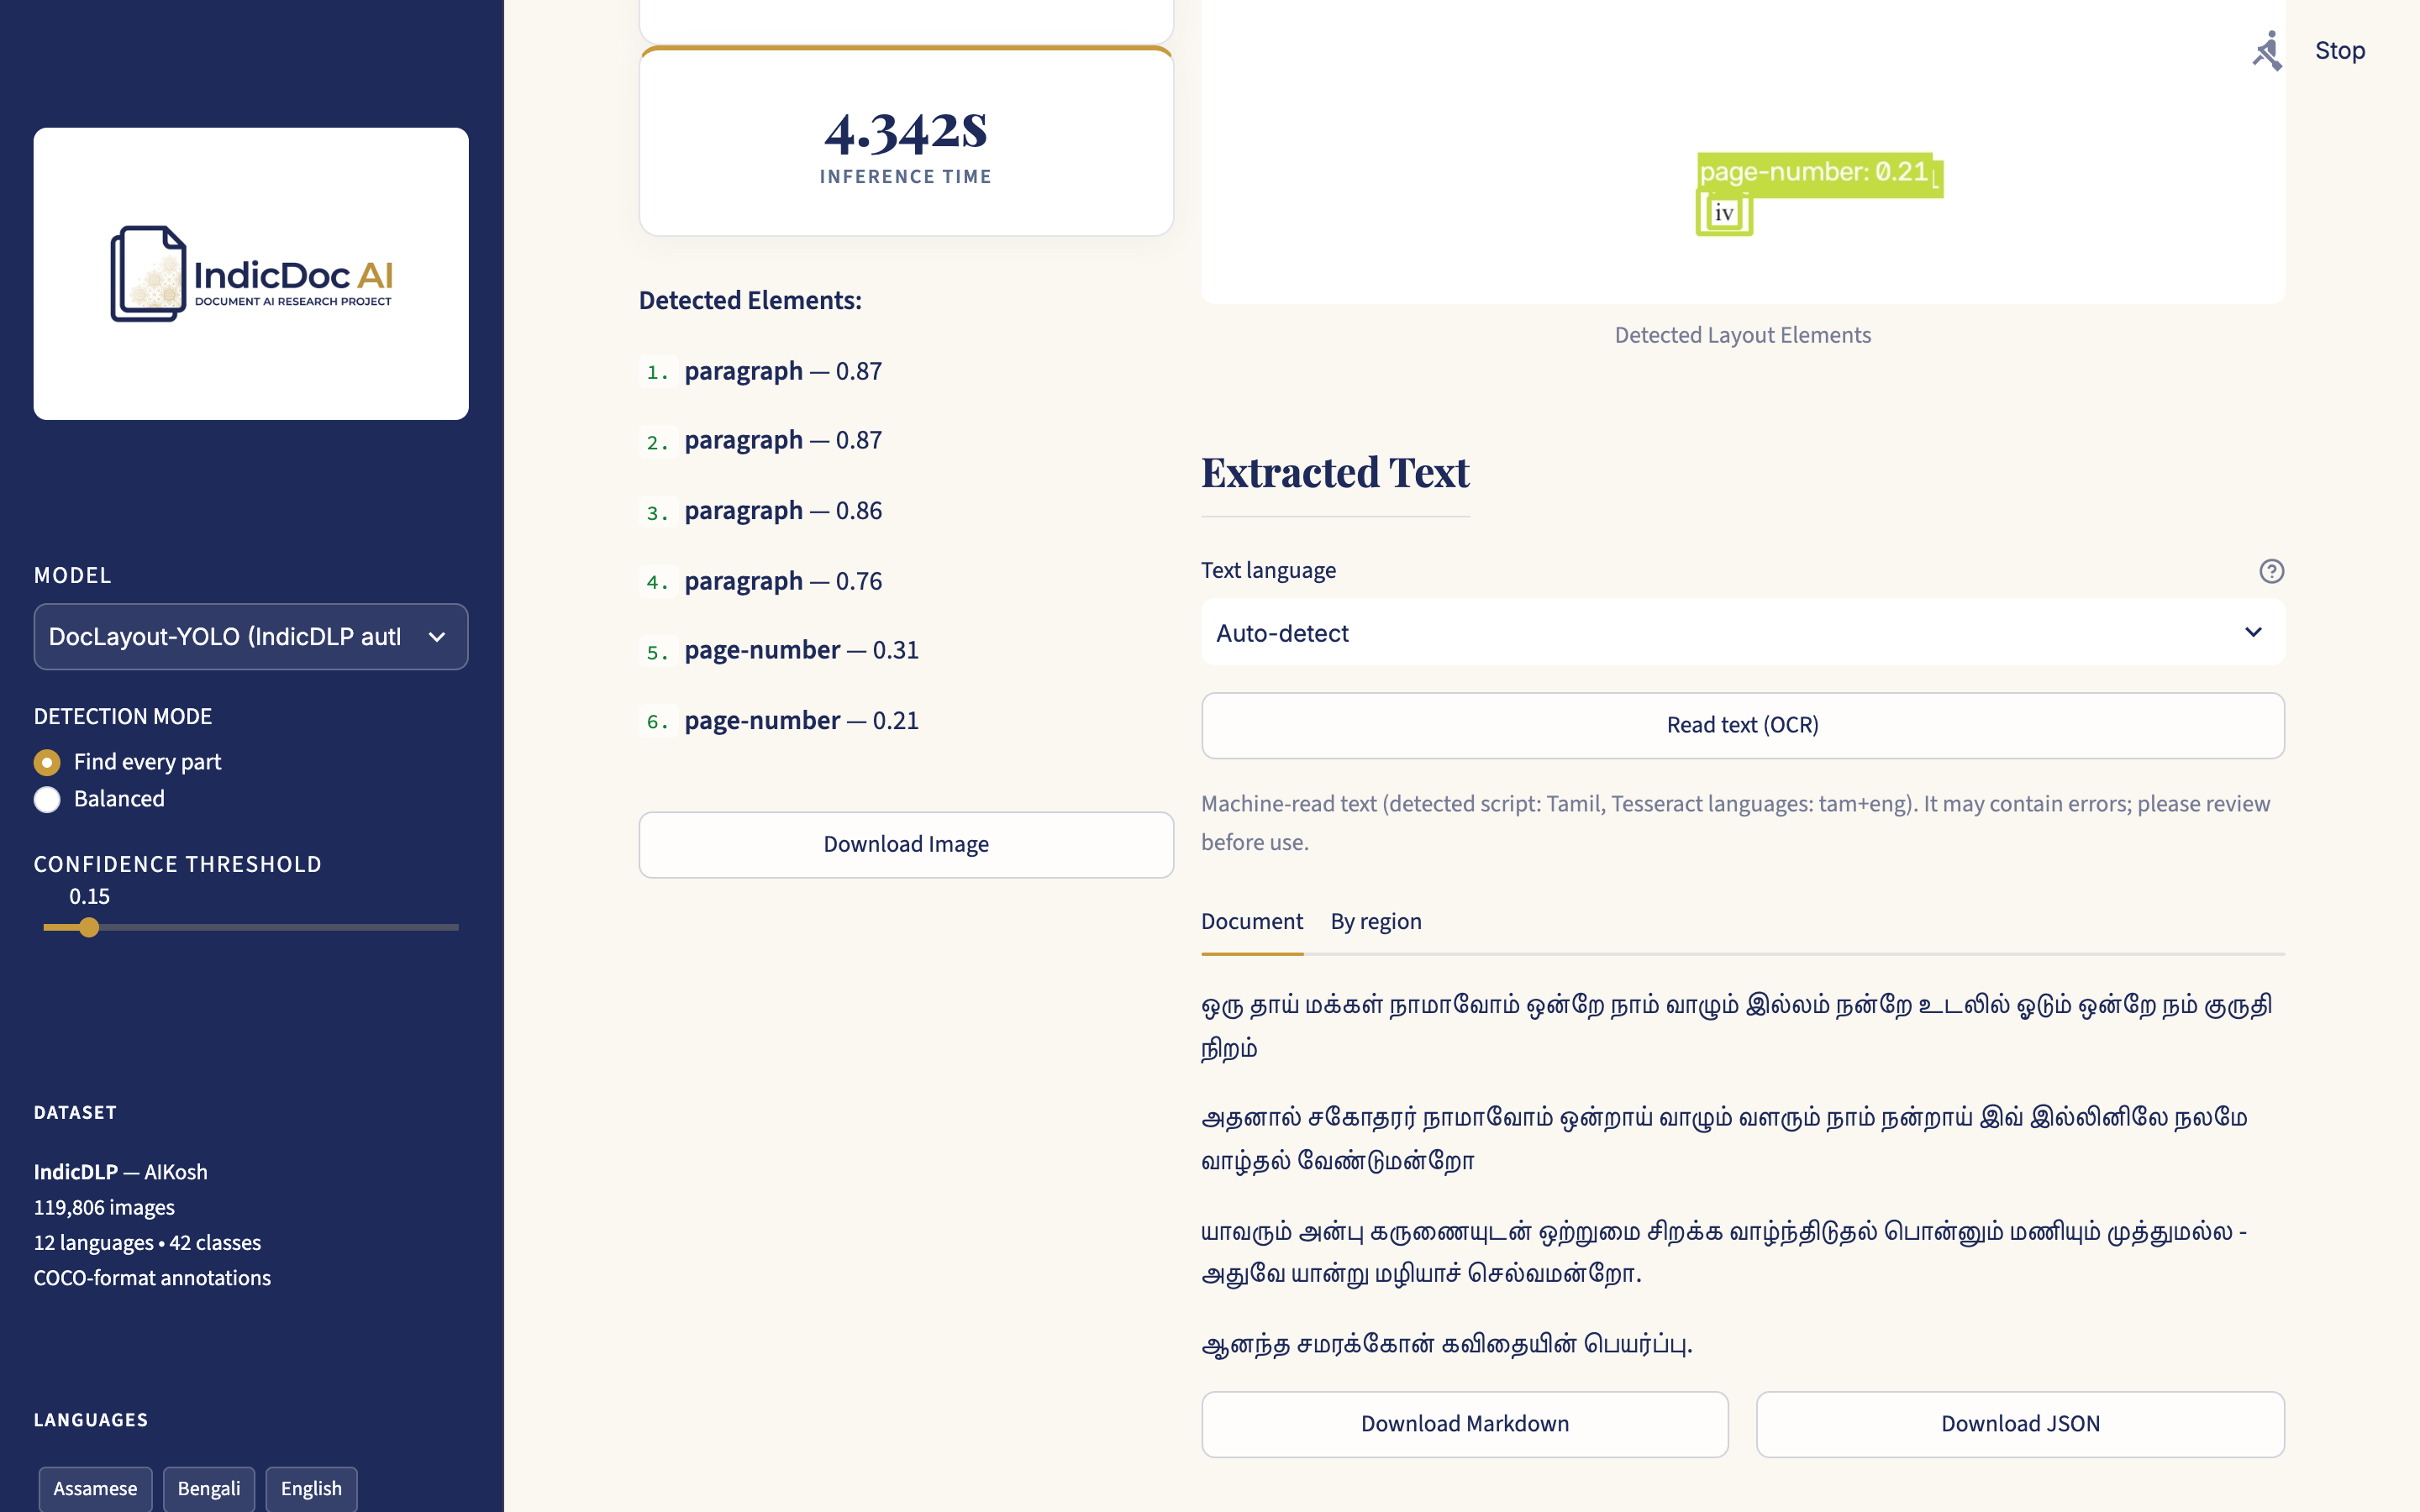
\includegraphics[width=\columnwidth]{figures/app_ocr.png}
\caption{IndicDoc AI on a Tamil textbook page: detected regions (left list) and the text read in reading order
with the script chosen automatically.}
\label{fig:app}
\end{figure}

\section{Discussion and Limitations}
\textbf{What the study suggests.} For someone who wants to process Indian documents, the choice of
\emph{document type} and \emph{scan quality} matters more than the language, once the script has been seen in
training. Forms, magazines and damaged pages are where effort should go: more labelled forms, and damage
augmentation during training. Simple ratios such as CI and RI make these weak spots visible in a way a
single mAP number does not.

\textbf{Limitations.} (1) We use a subset of 682 test pages; Hindi has only 22 of them, so its
numbers are less certain. (2) Our own models were trained for about an hour on a laptop GPU with one random seed, and the robustness test covers the released model and our YOLOv8s only. (3) Scan damage was simulated;
real damage often combines several kinds at once. (4) IndicDLP has no text ground truth, so we could not measure
OCR character accuracy; we measured only script choice and how much text falls inside regions. (5) The released
detector was trained by the IndicDLP authors; we evaluate it but did not train it.

\section{Conclusion}
We studied where layout detectors fail on Indian-language documents instead of proposing a new detector. On
682 IndicDLP test pages, the released DocLayout-YOLO is accurate (0.759 mAP@50) and fairly even across
the 12 languages, but much weaker on forms than on research papers, and it loses part of its accuracy on damaged
scans, most of all to blur. Choosing the OCR script by probing detected regions is far more reliable than
Tesseract's own detector. Future work: a controlled test of scripts never seen in training (same data size, with and without a script family), damage augmentation, more labelled forms, a stronger Indic OCR model with
a small text ground-truth set, and table structure and question answering on the detected tables. The code, the
data subset as CSV files and the tool are available to reviewers on request.

\section*{Acknowledgment}
We thank our guide Dr.~Joanne Gomes and the Department of AIML, SFIT. We thank the IndicDLP authors for releasing
their dataset and model.

\begin{thebibliography}{99}
\bibitem{indicdlp} O.~Nath, S.~Kukkala, M.~Khapra and R.~K.~Sarvadevabhatla, ``IndicDLP: A foundational dataset for multi-lingual and multi-domain document layout parsing,'' in \emph{Proc. ICDAR}, 2025, pp.~23--39.
\bibitem{doclayout} Z.~Zhao, H.~Kang, B.~Wang and C.~He, ``DocLayout-YOLO: Enhancing document layout analysis through diverse synthetic data and global-to-local adaptive perception,'' arXiv:2410.12628, 2024.
\bibitem{unitabbank} A.~Mondal \emph{et al.}, ``UniTabBank: A large scale multi-lingual, multi-layout, multi-type, multi-format dataset for table detection,'' in \emph{Proc. IEEE/CVF WACV}, 2026, pp.~6486--6495.
\bibitem{fasterrcnn} S.~Ren, K.~He, R.~Girshick and J.~Sun, ``Faster R-CNN: Towards real-time object detection with region proposal networks,'' in \emph{Proc. NeurIPS}, 2015.
\bibitem{yolov8} G.~Jocher, A.~Chaurasia and J.~Qiu, ``Ultralytics YOLOv8,'' 2023. [Online]. Available: \url{https://github.com/ultralytics/ultralytics}
\bibitem{platter} B.~V.~Kasuba, D.~Kudale, V.~Subramanian, P.~Chaudhuri and G.~Ramakrishnan, ``PLATTER: A page-level handwritten text recognition system for Indic scripts,'' arXiv:2502.06172, 2025.
\bibitem{hindiocr} S.~Bhattacharyya, S.~Ghosh, P.~Deb, A.~Mondal and C.~V.~Jawahar, ``Adapting vision-language models for Hindi OCR,'' IIIT Hyderabad, 2025.
\bibitem{layoutxlm} Y.~Xu \emph{et al.}, ``LayoutXLM: Multimodal pre-training for multilingual visually-rich document understanding,'' arXiv:2104.08836, 2021.
\bibitem{drishtikon} B.~V.~Kasuba, P.~Chaudhuri and G.~Ramakrishnan, ``DRISHTIKON: Visual grounding at multiple granularities in documents,'' arXiv:2506.21316, 2025.
\bibitem{tableqa} V.~Pal, E.~Kanoulas, A.~Yates and M.~de~Rijke, ``Table question answering for low-resourced Indic languages,'' arXiv:2410.03576, 2024.
\bibitem{devtables} A.~R.~Dumada and S.~G.~Shah, ``Incorporate structure and content for Devanagari table extraction,'' \emph{IJSAT}, vol.~17, no.~1, 2026.
\bibitem{hendrycks} D.~Hendrycks and T.~Dietterich, ``Benchmarking neural network robustness to common corruptions and perturbations,'' in \emph{Proc. ICLR}, 2019.
\bibitem{coco} T.-Y.~Lin \emph{et al.}, ``Microsoft COCO: Common objects in context,'' in \emph{Proc. ECCV}, 2014.
\bibitem{tesseract} R.~Smith, ``An overview of the Tesseract OCR engine,'' in \emph{Proc. ICDAR}, 2007.
\end{thebibliography}

\end{document}
